\section{Parameter Passing}

\begin{concept}{Parameter Passing Methods}\\
Data can be passed between functions through:
\begin{itemize}
  \item \textbf{Registers}: Fast, limited number available
  \item \textbf{Global Variables}: Shared memory space
  \item \textbf{Stack}: 
    \begin{itemize}
      \item Caller: PUSH parameters onto stack
      \item Callee: Access via LDR from stack
    \end{itemize}
\end{itemize}
\end{concept}

\begin{definition}{ARM Procedure Call Standard}\\
\textbf{Parameter Passing:}
\begin{itemize}
  \item First four arguments use R0-R3
  \item Additional parameters go on stack
\end{itemize}

\textbf{Return Values:}
\begin{itemize}
  \item \textbf{Small Values} ($\leqslant$ 32 bits): 
    \begin{itemize}
      \item Return in R0
      \item Zero/sign extend if needed
    \end{itemize}
  \item \textbf{Double Word} (64 bits): R0/R1
  \item \textbf{128-bit Values}: R0-R3
  \item \textbf{Larger Values}: 
    \begin{itemize}
      \item Store in memory
      \item Return pointer in R0
    \end{itemize}
\end{itemize}

\textbf{Register Usage:}
\begin{itemize}
  \item \textbf{R0-R3}: Arguments/results (caller-saved)
  \item \textbf{R4-R11}: Local variables (callee-saved)
  \item \textbf{R12}: IP - scratch register
  \item \textbf{R13}: SP - stack pointer
  \item \textbf{R14}: LR - link register
  \item \textbf{R15}: PC - program counter
\end{itemize}

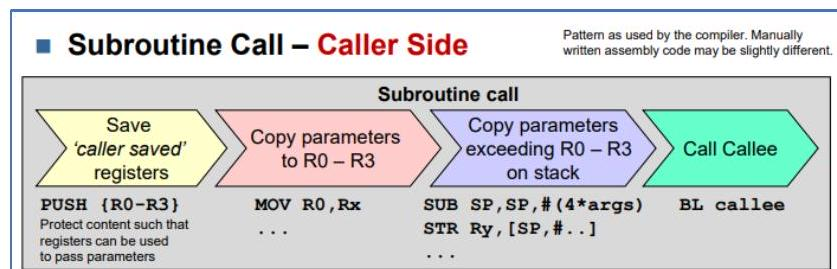
\includegraphics[width=\linewidth]{images/2024_12_29_79e6b22f503fb7b4f718g-09(3)}
\end{definition}

\begin{concept}{Reentrancy}\\
Handling recursive function calls:
\begin{itemize}
  \item Each call needs its own data set
  \item Registers/globals get overwritten
  \item Solution: Use stack for local storage
\end{itemize}
\end{concept}

\begin{example2}{Parameter Passing Methods}
Global variable approach (not recommended):
\begin{lstlisting}[language=armasm, style=basesmol]
    .data
value   DCD     0           ; Global variable

    .text
func    LDR     R0, =value  ; Load address
        LDR     R1, [R0]    ; Get value
        ; Process value
        STR     R1, [R0]    ; Store result
\end{lstlisting}

Register-based approach (preferred):
\begin{lstlisting}[language=armasm, style=basesmol]
func    PUSH    {R4, LR}    ; Save registers
        ; R0 contains input parameter
        MOV     R4, R0      ; Save parameter
        ; Process value in R4
        MOV     R0, R4      ; Set return value
        POP     {R4, PC}    ; Restore and return
\end{lstlisting}
\end{example2}

\begin{KR}{Implementing Function Calls}\\
Steps for calling functions:
\begin{enumerate}
  \item Caller's responsibilities:
    \begin{itemize}
      \item Place parameters in R0-R3
      \item Push additional parameters on stack
      \item Save caller-saved registers if needed
    \end{itemize}
  \item Callee's responsibilities:
    \begin{itemize}
      \item Save callee-saved registers used
      \item Save LR if making other calls
      \item Process parameters
      \item Place return value in R0
      \item Restore saved registers
    \end{itemize}
\end{enumerate}
\end{KR}

\begin{remark}
Important considerations:
\begin{itemize}
  \item Avoid global variables for parameter passing
  \item Use registers for efficiency
  \item Follow ARM calling convention strictly
  \item Consider stack usage in recursive functions
\end{itemize}
\end{remark}